\documentclass[10pt]{article}

\usepackage[utf8]{inputenc}
\usepackage[francais]{babel}
\usepackage{multicol}
\usepackage{subfig}
\usepackage{float}
\usepackage{nonfloat}
\usepackage{tikz}

% FAMFAMFAM.com colors
\definecolor{mpink}{RGB}{255,11,91}
\definecolor{mblue}{RGB}{11,206,255}
\definecolor{mgreen}{RGB}{123,255,45}

\setlength{\textwidth}{39pc}
\setlength{\textheight}{50pc}
\setlength{\parindent}{1em}
\setlength{\parskip}{0pt plus 1pt}
\setlength{\oddsidemargin}{0pc}
\setlength{\marginparwidth}{0pc}
\setlength{\topmargin}{1pc}
\setlength{\headsep}{20pt}
\setlength{\columnsep}{2pc}

\title{Recherche décentralisée de connexité pour réseaux de capteurs mobiles}
\author{Merwan Achibet}
\date{}

\begin{document}

\maketitle

\begin{multicols}{2}

\section*{Introduction}

On traite le problème suivant : un groupe de $n$ capteurs mobiles est
réparti aléatoirement dans un espace aérien. On part de l'hypothèse
qu'un capteur connaît uniquement le nombre total de capteurs du
système et qu'il est assez sophistiqué pour pouvoir déterminer
précisément sa position absolue. Les capteurs sont dotés de matériel
de communication sans fil et peuvent s'envoyer des messages à
condition que la distance les séparant soit inférieure à leur rayon
d'émission $R_c$.

Le réseau constitué par cet essaim d'appareils volants forme un graphe
dynamique dont les n\oe uds sont les capteurs. Deux n\oe uds sont
reliés par un arc si les capteurs qui leur sont associés sont en
mesure de communiquer, c'est à dire s'ils sont assez proches. La
figure \ref{communication} décrit un exemple de scénario impliquant
trois capteurs.

\begin{figure}[H]

  \centering

  \begin{tikzpicture}

  \draw (0,0) -- (-1,1);

  \drawSensor{0}{0}{2}{red}
  \drawSensor{-1}{1}{2}{blue}
  \drawSensor{2.5}{1}{2}{green}

\end{tikzpicture}


  \caption{Les capteurs rose et bleu peuvent communiquer et sont
    connectés tandis que le capteur vert est isolé.}
  \label{communication}

\end{figure}

On considère un capteur comme un agent autonome capable de se mouvoir
dans l'espace. Afin de ne pas se préoccuper de considérations
géométriques superflues, il est supposé qu'un capteur conserve
toujours la même altitude et donc on limite son déplacement à deux
dimensions. La contrainte principale de cet exercice est que l'on
refuse toute forme de contrôle global sur l'essaim de capteurs. Toutes
les actions entreprises par un appareil seront uniquement dues à ses
décisions propres et dépendront de la vue réduite du système dont il
dispose.

La possibilité pour un capteur de communiquer avec ses semblables est
au centre de nos préoccupations car on considère qu'un capteur isolé
est inutile puiqu'incapable de partager des données. Dans le contexte
de l'étude décentralisée d'un graphe dynamique, deux questions se
posent :

\begin{enumerate}
\item{Comment déterminer si le réseau de capteurs est connexe ?}
\item{Comment déplacer les capteurs de façon à ce qu'il le devienne ?}
\end{enumerate}

Pour répondre à la première question, on se concentre sur les
communications de capteur à capteur en proposant une méthode pour
laquelle chaque agent diffuse sa vision de la connexité du réseau,
étiquettée en fonction de la date de chaque information et de son
origine. Un mécanisme de filtrage autorégulant sera mis en place pour
répandre les informations critiques telles que l'ajout d'un nouveau
n\oe ud à une composante connexe et stoppant la diffusion
d'informations erronnées.

La réponse à la seconde question s'attache à l'aspect mobile d'un
capteur. On propose une méthode décentralisée de guidage se basant sur
l'imitation de plusieurs lois physiques de la nature afin de former un
maillage à la fois connexe, équilibré et étalé dans
l'espace. Finalement, on envisage une extension de ce système pour
permettre aux capteurs d'éviter naturellement les obstacles.

\section{Déterminer si le réseau est connexe}

Dans cette section, on se place du point de vue d'un capteur $c$ et
l'on considère que le réseau est connexe lorsque $c$ le pense connexe.

Les capteurs étant mobiles, le réseau de communication qu'ils forment
est hautement dynamique et des événements impromptus, comme le
déplacement d'un capteur ou une panne, peuvent à tout moment faire
varier la connexité du graphe résultant. Comme énoncé précédemment,
$c$ a connaissance du nombre de capteurs $n$ du système. Déterminer la
connexité du réseau revient donc à un problème de comptage
décentralisé, o\`u $\tilde{n}$ est le nombre de capteurs que $c$ sait
connectés à sa propre composante connexe, et le graphe est connexe si
$\tilde{n} = n$.

L'idée que l'on présente ici repose sur un partage permanent, entre
voisins, de la vision du réseau que chaque capteur entretient. Si l'on
pouvait traduire en langue humaine un message de $c$ à $c'$, on
entendrait :

\begin{quote}
  \textit{Je suis $c$ et $c'$ m'a dit que $x$ à été vu dans le réseau
    il y a 14 secondes. Par contre, je n'ai pas eu de nouvelles de mon
    voisin $y$ depuis 78 secondes, je doute du fait qu'il soit
    toujours présent dans le réseau.}
\end{quote}

Dans notre méthode, un capteur transmet régulièrement à ses voisins
son avis sur la présence ou non d'autres n\oe uds dans sa composante
connexe. Afin de permettre de gérer des informations potentiellement
contradictoires, une date et une source sont associées à chaque
information de n\oe ud. Par comparaison temporelle et par élagage des
informations fournies par les n\oe uds eux-mêmes déconnectés, on
provoque dans le réseau une dynamique globale de comptage qui se
stabilise lorsque le graphe devient connexe. On précise par la suite
les trois structures de données qui serviront de support à ces
échanges.

Puisque le filtrage par comparaison d'informations contradictoires se
base sur une donnée temporelle, on suppose que les capteurs disposent
d'une horloge interne et qu'ils sont synchronisés. On suppose aussi
qu'ils possèdent une mémoire interne afin de stocker les trois
structures de données décrites ci-dessous.

\subsection*{Données propres à un capteur}

Chaque capteur entretient trois listes de données. On décrit d'abord
la nature de leur contenu puis l'on développe la façon dont ce contenu
est acquis dans la section suivante.

La première liste, $N$, représente le voisinage de $c$ et contient
uniquement les identifiants des n\oe uds en liaison directe avec ce
dernier.

La seconde liste entretenue par un capteur est $C$. Elle représente sa
vision de la connexité du réseau, soit concrètement, tous les n\oe uds
qui, de son point de vue, y sont connectés directement (par voisinage)
ou indirectement (par l'intermédiaire d'autres capteurs). On en déduit
que tous les n\oe uds représentés dans $N$ apparaissent dans
$C$. Contrairement à $N$, $C$ ne contient pas que des identifiants et
ses entrées sont des triplets $(c',t,s)$ avec $c'$ l'identifiant du
n\oe ud dont l'on veut exprimer la présence sur la composante connexe,
$t$ le dernier temps auquel $c'$ a été détecté et $s$ le capteur ayant
transmis cette information à $c$ (la \textit{source}).

La troisième et dernière liste, $D$, contient les capteurs dont $c$
n'est plus certain de la connexité. Ses entrées prennent la forme de
paires $(c',t)$ o\`u $c'$ est le n\oe ud sur lequel le doute se pose
et $t$ la date à laquelle l'absence de $c'$ a été dernièrement
remarquée.

\subsection*{Modification autonome de l'état interne}

Les trois listes décrivant la connaissance du réseau dont dispose un
capteur ont été présentées mais la question de l'origine des
informations qu'elles contiennent n'a pas encore été abordée. On se
concentre dans un premier temps sur les modifications qu'un capteur
applique à sa propre mémoire à partir de ses propres observations.

Afin de présenter le plus clairement possible ce problème, on imagine
la situation d'un capteur $c$ fraîchement arrivé dans le système et
n'ayant encore rencontré aucun autre n\oe ud.

Si $c$ reçoit un message d'un capteur $c'$, il l'ajoute à sa liste de
voisins $N$ ainsi qu'à sa liste de connexité $C$ tout en y associant
une date et une source adaptées (ici la source est simplement
$c'$). La liste $N$ n'est jamais partagée avec les autres capteurs
mais permet à $c$ de disposer d'une liste séparée contenant uniquement
ses voisins directs.

On choisit d'aborder le problème de façon proactive : les messages
d'un capteur sont envoyés volontairement et à intervalle régulier afin
d'informer ses voisins de sa présence. Ainsi, on considère qu'un
capteur a potentiellement disparu d'un voisinage s'il n'envoie plus de
message; ou plus précisément, si les voisins l'ayant enregistré n'en
ont plus de nouvelle depuis un certain temps. C'est le processus de
\textit{surveillance}.

Ainsi, si $c$ ne reçoit plus de message de $c'$ pendant un certain
temps, il supprimera toute référence à $c'$ de ses listes $N$ et $C$
et l'ajoutera $D$, la liste des doutes. Le changement de statut de
$c'$ n'est pas définitif et s'il se connecte à nouveau à $c$,
l'opération inverse sera effectuée.

\subsection*{Modition de l'état interne par propagation des rumeurs}

les modifications de la mémoire décrites concernaient uniquement le
domaine dont un capteur $c$ est certain, son voisinage. On évoque
maintenant la façon dont toutes les informations sont diffusées dans
le réseau afin de comprendre comment un capteur situé à un de ses
bouts prend connaissance de sa connexité avec un capteur placé à
l'autre bout.

On a suggéré qu'un capteur prend connaissance de la présence d'un
voisin en recevant ses messages sans pour autant préciser leur
nature. Un message est en fait constitué des listes $C$ et $D$ de son
émetteur. \`A la réception de ces données, un capteur $c$ va traiter
ces listes et évaluer quelles informations retenir et quelles autres
informations ignorer en se basant sur les étiquettes temporelles.

Par exemple, si $c$ reçoit de $c'$ la liste $C' =
\{\dots,(x,23,y),\dots\}$ et que le capteur $x$ ne fait partie
d'aucune des listes de $c$, alors il l'absorbe et $C =
\{\dots,(x,23,c')\}$. On remarque que la source de l'information est
modifiée car c'est $c'$ qui a transmis l'information à $c$ et $y$ n'a
joué aucun rôle dans cet échange.

Autre exemple, $c$ possède $C = \{\dots,(x,23,y),\dots\}$ et $c'$ lui
transmet $C' = \{\dots,(x,37,z),\dots\}$. Le même capteur $x$ est
présent à la fois dans la liste de connexité de $c$ et dans celle de
$c'$ ce qui signifie que chacun de ces deux n\oe uds admet que $x$
fait partie de leur composante connexe. Par contre, la date associée à
la dernière détection de $x$ est plus récente du côté de $c'$ donc on
la met à jour dans $c$. On a au final $C = \{\dots,(x,37,c'),\dots\}$.

La liste de doutes $D$ n'est pas encore entrée en jeu mais elle aussi
joue un rôle important. Par exemple, $c$ a $C =
\{\dots,(x,42,y),\dots)\}$ et reçoit de $c'$ la liste $D' =
\{\dots,(x,56,z),\dots\}$. Puisque $c'$ dispose d'une information plus
récente établissant que $x$ n'est plus présent dans le système depuis
le temps 56, alors on lui fait confiance et $D =
\{\dots,(x,56,c'),\dots\}$ tandis que la référence à $x$ est retirée
de $C$.

De plus, $c$ peut être amené à réfuter une partie de ses connaissances
s'il s'aperçoit qu'un n\oe ud qui en est à l'origine (qui en est la
source donc) est mis en doute de façon crédible par un voisin. Prenons
l'exemple de $C = \{\dots,(x,14,y),(y,5,z),\dots\}$ et $D' =
\{\dots,(y,20,w),\dots\}$. Comme pour l'exemple précédent, les deux
capteurs ont un avis différent sur la présence de $y$ dans le système
et c'est $c'$ qui l'emporte car son information est plus récente. On
passe donc $y$ de $C$ à $D$ tout en mettant à jour la date de
l'observation et la source de l'information. En plus de cette
modification, on retire $(x,14,y)$ de $C$ car $y$, qui vient d'être
jugé comme déconnecté, en est la source. C'est ce procédé de
rétrodiffusion qui permet le comptage dans un graphe dynamique car par
propagation toutes les connaissance du réseau ayant $y$ comme source
vont être réévaluées.

Ces quelques exemples illustrent l'idée de cette méthode de comptage
décentralisée basée sur le constat que seuls les voisins directs
peuvent affirmer avec certitude la présence ou non d'un capteur dans
leur voisinage. Pour connaître l'état des n\oe uds distants, on compte
sur la diffusion des données de connexité et le filtrage annulant les
connaissance potentiellement fausses. Un exemple graphique est visible
sur la figure \ref{connexite}.

Cet algorithme fournit uniquement une approximation de la connexité du
réseau car les informations souffrent d'un temps de propagation
proportionnel à la distance entre le capteur observant la modification
de son voisinage et le capteur recevant plus tard l'information passée
de mains en mains. De plus, une fréquence d'émission trop élevée est
encline à générer des \textit{broadcast storms} dans une situation
réelle. Néanmoins, cette méthode permet l'évaluation de la connexité
d'un graphe dynamique.

\section{Rendre le réseau connexe}

On traite maintenant la seconde interrogation soulevée par ce problème
: comment déplacer les capteurs pour obtenir un réseau connexe ?

La résolution de ce problème passe par la satisfaction de deux besoins
\textit{a priori} antagonistes. D'une part, il est naturellement
nécessaire de réunir les capteurs dans un espace réduit, de façon à ce
qu'ils puissent communiquer et échanger des données en
continu. D'autre part, et dans l'interêt de leurs utilisateurs, ils
doivent s'étaler dans l'espace afin d'effectuer des mesures sur la
plus grande superficie possible. Nous sommes donc dans une situation
de compromis, dans laquelle une contrainte technique (la portée de
communication) force à agglomérer les capteurs en une même zone,
tandis que leur but premier est de relever des données en masse et
donc, rationnellement, de s'éloigner les uns des autres pour couvrir
le plus de terrain possible. La seule issue favorable à ce problème
est donc d'aboutir à une situation d'équilibre satisfaisant ces deux
contraintes diamétralement opposées.

Le cadre de cet exercice s'accorde parfaitement avec la problèmatique
de la prise de décision dans un réseau décentralisé puisque chaque
capteur peut être assimilé à un agent autonome, capable d'agir sur la
configuration de son environnement en se déplaçant dans l'espace. Quel
que soit l'état d'un capteur, la vision du système dont il dispose est
locale et doit servir seule à déterminer quelles actions il
entreprend. L'objectif est donc ici de proposer une méthode de guidage
que chaque capteur peut adopter et qui, par émergence d'une dynamique
globale, résout notre problème en répartissant les capteurs dans
l'espace de façon satisfaisante.

Les boïds de Craig Reynolds \cite{Reynolds1987} sont reconnus pour
simuler un comportement d'apparence complexe et synchronisée à partir
d'un jeu de règles simples. On s'en inspire, ainsi que d'un modèle de
mouvement particulaire \cite{Cheng2011497} se basant sur la répulsion
entre molécules de gaz, pour concevoir les trois règles qui
gouverneront notre système. Chacune de ces lois, que l'on présente
séparément par la suite, engendre une influence sur le déplacement de
nos capteurs; influence dont la composition sera détaillée en dernière
partie.

\subsection*{Attraction}

\`A la lecture de l'énoncé de ce problème, la nécessité de rapprocher
les capteurs les uns des autres, afin qu'un réseau de communication
ininterrompu se forme, vient naturellement à l'esprit. En effet, la
condition \textit{sine qua non} au bon fonctionnement du réseau est la
communication.

Par sa loi de la gravitation universelle, Isaac Newton décrit la force
qui attire toute paire de corps comme étant proportionnelle à leur
masse respective et à la distance les séparant \cite{newton}. Nous
nous permettons de simplifier quelque peu son équation et d'en retirer
l'aspect massique pour obtenir une règle qui a tout couple de corps
associe une attraction proportionnelle à leur distance. S'ils
obéissaient à cette loi, nos capteurs auraient naturellement tendance
à se grouper.

\`A l'échelle de notre système, le cadre est différent de celui de la
loi de Newton, et cette influence n'est pas universelle. Nous ne
pouvons malheureusement pas réécrire les règles de ce monde et
inventer une attirance magique entre toute paire de capteurs. On peut
néanmoins la simuler. Si deux capteurs sont à portée de communication
et peuvent échanger leur position respective alors la détermination de
la distance les séparant est aisée et la simulation d'un phénomène
d'attraction devient possible.

Concrètement, on associe à tout capteur $c$ un rayon d'attraction
$R_a$ (voir figure \ref{attraction}). Si un capteur voisin se trouve à
la fois dans le rayon de communication $R_c$ de $c$ et à l'extérieur
de $R_a$, la force d'attraction que ce capteur subit est :

$$
\vec{a} = \frac{\vec{p}_c - \vec{p}_v}{|\vec{p}_c - \vec{p}_v|^2}
$$

\begin{figure}[H]

  \centering

  \begin{tikzpicture}

  \drawSensor{0}{0}{2}{black}
  \draw (0,0) circle (1.5);

  \draw[fill=black] (200:1.8) circle (0.1);
  \draw[->] (200:1.8) -- (200:1);

\end{tikzpicture}


  \caption{En pointillés verts, le rayon d'attraction, dont
    l'intensité est décroissante de l'intérieur vers l'extérieur.}
  \label{attraction}

\end{figure}

Dans le phénomène d'attraction réel, l'action est réciproque et
instantanée mais dans notre cas elle est unidirectionnelle. Un capteur
est attiré par tous ses voisins mais le processus décrit ne modifie
pas directement la position du voisin en question et il n'en subit
aucune influence. Il est néanmoins à prévoir que lorsque ce voisin
calculera les influences qui s'appliquent à lui, il en subira la
réciproque.

On note que l'attraction n'a pas pour but d'approcher des capteurs
trop éloignés pour communiquer puisque l'existence d'une connexion
entre deux capteurs est un prérequis à l'application de la force
d'attraction. Son interêt majeur est de renforcer l'assurance d'une
communication pérenne et un effet secondaire appréciable se révélera
par association avec la seconde force présentée.

\subsection*{Répulsion}

L'attraction a pour effet d'agglomérer en groupes serrés tous les
capteurs démarrant la simulation dans une même zone. Mais même si de
cette façon la communication est assurée, les capteurs finissent par
être réunis en une zone très réduite au bout d'un certain nombre
d'itérations et la contrainte de couverture n'est absolument pas
satisfaite.

Pour pallier cette déconvenue, on introduit une nouvelle force opposée
à l'attraction, la répulsion. Le rayon $R_r$ définit une nouvelle zone
radiale qui, contrairement à la loi précédente, expulsera les capteurs
envahissants vers l'extérieur. L'influence qui en découle est
inversement proportionnelle à la distance les séparant, de façon à
engendrer une répulsion plus forte vers le centre \cite{Cheng2011497}
:

$$
\vec{r} = \frac{\vec{p} - \vec{p_v}}{|\vec{p} - \vec{p_v}|}(R_r - |\vec{p} - \vec{p_v}|)
$$

\begin{figure}[H]

  \centering

  \begin{tikzpicture}

  \drawSensor{0}{0}{2}{black}
  \draw (0,0) circle (1.5);

  \draw[fill=black] (150:0.5) circle (0.1);
  \draw[->] (150:0.5) -- (150:1.3);

\end{tikzpicture}


  \caption{En pointillés rouges, le rayon de répulsion, dont
    l'intensité est décroissante du centre vers les bords.}
  \label{repulsion}

\end{figure}

On prend $R_r = R_a - \varepsilon$, o\`u $\varepsilon$ correspond à la
largeur d'une bande neutre entourant chaque capteur (voir figure
\ref{repulsion}). Les capteurs auront naturellement tendance à
s'installer dans ces zones libre de toute influence. Nous verrons dans
les démonstrations que la conséquence principale de ce positionnement
fortement dirigé est une organisation en un maillage régulier et
géométrique. La régularité qu'adopte la structure de notre réseau est
un plus à ne pas négliger puisqu'il permet des mesures de
l'environnement homogènes.

\subsection*{Gravité}

Les deux règles présentées permettent aux capteurs de s'agglomérer en
composantes connexes équilibrées mais ces composantes prennent la
forme d'îlots séparés et la connexité totale du réseau n'est toujours
pas garantie. Dans cette optique, on introduit une dernière influence
inspirée de la physique, la gravité.

Comme annoncé en introduction, on part de l'hypothèse que les capteurs
sont munis de moyens de localisation dans l'espace et nous en avons
jusque là allègrement profité pour les calculs de distance nécessaires
à l'évaluation des forces. Dans la continuité de cette hypothèse, on
peut supposer que tous les capteurs connaissent le centre géométrique
de l'environnement dans lequel ils évoluent. Cette position peut être
la position de laquelle ils ont été largués, une position
pré-programmée ou un point calculée de façon décentralisée par moyenne
de toutes leur positions. La notion importante est que cette position
est connue de tous et sert d'origine à leur système de coordonnées.

La gravité est la force qui va attirer tous les capteurs vers le
centre de l'environnement. \`A première vue, une telle règle semble
dangereuse car on imagine qu'elle poussera les capteurs à se déplacer
vers le centre de la zone au risque de sacrifier l'étendue de la zone
couverte. Néanmoins, on compte sur l'effet combiné des différentes
forces, notamment la répulsion, pour résister à ce phénomène.

L'interêt de la gravité est d'attirer vers un même espace les capteurs
isolés et les composantes connexes chanceuses formées par l'attraction
et équilibrées par la répulsion. On la calcule de façon uniforme,
comme un vecteur unitaire dirigé vers le centre de l'environnement.

$$
\vec{g} = -\frac{\vec{p}}{|\vec{p}|}
$$

\begin{figure}[H]

  \centering

  \begin{tikzpicture}

  \node[path picture={
      \draw[black] (path picture bounding box.south east) -- (path
      picture bounding box.north west);
      \draw[black] (path picture bounding box.north east) -- (path
      picture bounding box.south west);}] at (0,0) {};

  \draw[fill=black] (120:3) circle (0.1);
  \draw[->] (120:3) -- (120:2.5);

  \draw[fill=black] (180:3) circle (0.1);
  \draw[->] (180:3) -- (180:2.5);

  \draw[fill=black] (10:3) circle (0.1);
  \draw[->] (10:3) -- (10:2.5);

\end{tikzpicture}


  \caption{La gravité attire tous les capteurs vers le centre de
    l'environnement.}
  \label{gravite}

\end{figure}

\subsection*{Composition d'une force nette}

Une fois ces trois forces évaluées, on ne peut pas les appliquer
naïvement sur le capteur concerné car il s'agit d'un objet physique
soumis à des limitations quant à sa vitesse de déplacement. On associe
donc à chaque capteur une vitesse maximale qui sert de borne
supérieure à la magnitude des trois forces combinées.

Puisque l'on dispose de trois influences différentes, chacune tenant
un rôle particulier dans la résolution du problème, l'idée la plus
intuitive est d'en déduire une influence moyenne.

$$
\vec{f} = \frac{\vec{a} + \vec{r} + \vec{g}}{3}
$$

En pratique, ce choix montre vite ses limites. En effet, sous
certaines configurations, deux forces peuvent prendre des directions
opposées et les combiner de la sorte annule tout mouvement. Or
l'inaction est rarement une solution. Dans d'autres cas relativement
fréquents, les trois forces semblents correctement pondérées : on
observe des capteurs isolés flotter lentement vers le centre de leur
environnement et s'assembler en composantes connexes de plus en plus
grandes. Mais une fois que le maillage est complet et qu'une situation
d'équilibre semble avoir été atteinte, le centre du réseau commence à
trembler; les capteurs centraux se rapprochent dangereusement et se
superposent sur l'origine de l'univers, ignorant totalement la règle
de répulsivité. Ce problème est du à la quantité importante de
tensions s'opérant au centre du réseau. La pression intense qui en
résulte fait s'effondrer le réseau jusqu'à ce que tous les capteurs
occupent la même position. Moyenner les forces est donc une fausse
bonne idée.

On préférera prioritiser les forces, c'est à dire leur donner un ordre
d'importance. Le mode opératoire est le suivant :

\begin{enumerate}
\item{On définit l'ordre des forces, dans notre cas répulsion puis
  attraction puis gravité.}
\item{On calcule la force de répulsion et on l'applique en bornant par
  la vitesse maximale des capteurs.}
\item{S'il reste de la marge de man\oe uvre, on recommence cette
  opération avec l'attraction.}
\item{S'il reste de la marge de man\oe uvre, on recommence cette
  opération avec la gravité.}
\end{enumerate}

De cette façon, les situations d'urgence telles que l'écartement
rapide de deux capteurs trop proches prennent le pas sur des
mouvements de composition, tels que celui d'un capteur isolé flottant
vers l'origine. Ce procédé est appliqué aux boïds de Reynolds pour
prioritiser l'évitement d'obstacles face aux forces de cohésion du
groupe. Une succession d'étapes menant à la formation d'un réseau
connexe est visible sur la figure \ref{demo}.

Pour prouver la versatilité de notre système, on propose finalement
d'étendre ce modèle de guidage afin de permettre aux capteurs d'éviter
automatiquement les obstacles par l'ajout d'une nouvelle force
virtuelle. Un obstacle représente toute zone non traversable. Il peut
s'agir d'un bâtiment, d'une zone dont les relevés ne nous intéressent
pas ou d'un espace interdit aux appareils volants. Dans un soucis de
simplicité (et de délais !), on limite les obstacles à des formes
circulaires afin de mieux s'accorder avec l'aspect radial des
différentes forces introduites jusqu'à présent.

Une force de répulsion du même type que celle éloignant les capteurs
les uns des autres est appliquée sur chaque obstacle et est
inversement proportionnelle à la distance entre le capteur soumis à la
force est l'obstacle, afin de provoquer des expulsions rapides. Lors de
la composition des différentes forces que subit le capteur, on choisit
d'appliquer en priorité la nouvelle force d'évitement des obstacles,
avant même la répulsion. La figure \ref{obstacles} illustre le
comportement obtenu.

\begin{figure}[H]

  \centering

  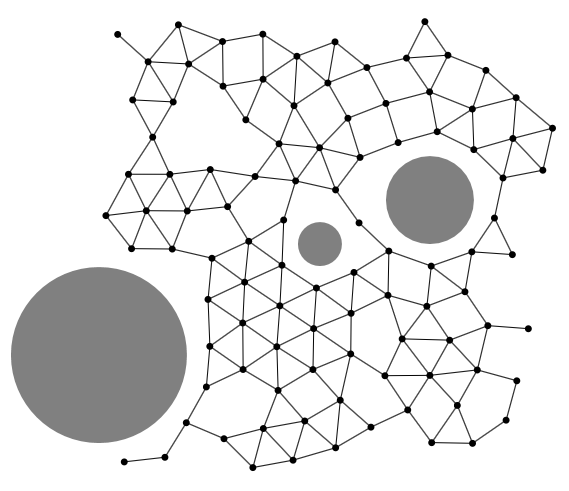
\includegraphics[width=7cm]{obstacles.png}

  \caption{Réseau connexe obtenu dans un environnement à obstacles.}
  \label{obstacles}

\end{figure}

\section*{Conclusion}

\end{multicols}

\begin{figure}[p]

  \centering

  \subfloat[\underline{$t$ = 0} Les capteurs sont éloignés et ne sont
    pas en mesure de communiquer. Aucun capteur n'a connaissance des
    autres capteurs du système.]{\begin{tikzpicture}

  \draw (180:2) node[draw,circle,fill=white] (a) {A};
\draw (270:1) node[draw,circle,fill=white] (d) {D};
\draw (0:2) node[draw,circle,fill=white] (c) {C};
\draw (90:1) node[draw,circle,fill=white] (b) {B};


  \draw (0,1.8) node {$D = \{\}$}
  ++(0,0.5) node {$C = \{\}$}
  ++(0,0.5) node {$N = \{\}$};

  \draw (2.3,0.7) node {$D = \{\}$}
  ++(0,0.5) node {$C = \{\}$}
  ++(0,0.5) node {$N = \{\}$};

  \draw (0,-2.8) node {$D = \{\}$}
  ++(0,0.5) node {$C = \{\}$}
  ++(0,0.5) node {$N = \{\}$};

  \draw (-2.3,0.7) node {$D = \{\}$}
  ++(0,0.5) node {$C = \{\}$}
  ++(0,0.5) node {$N = \{\}$};

\end{tikzpicture}
}\\

  \vspace{5cm}

  \subfloat[\underline{$t$ = 1} Les capteurs B, C et D sont assez
    proches pour communiquer. C émet un message. B et D intègrent
    ses informations.]{\begin{tikzpicture}

  \draw (180:2) node[draw,circle,fill=white] (a) {A};
\draw (270:1) node[draw,circle,fill=white] (d) {D};
\draw (0:2) node[draw,circle,fill=white] (c) {C};
\draw (90:1) node[draw,circle,fill=white] (b) {B};


  \draw[thick] (b) -- (c);
  \draw[thick] (c) -- (d);

  \draw (0,1.8) node {$D = \{\}$}
  ++(0,0.5) node {$C = \{(C,3)\}$}
  ++(0,0.5) node {$N = \{C\}$};

  \draw (2.3,0.7) node {$\{\}$}
  ++(0,0.5) node {$\{(C,3)\}$}
  ++(0,0.5) node {$\{C\}$};

  \draw (0,-2.8) node {$\{\}$}
  ++(0,0.5) node {$\{(C,3)\}$}
  ++(0,0.5) node {$\{C\}$};

  \draw (-2.3,0.7) node {$\{\}$}
  ++(0,0.5) node {$\{(C,3)\}$}
  ++(0,0.5) node {$\{C\}$};

\end{tikzpicture}
}

  \caption{}
  \label{connexite}

\end{figure}

\begin{figure}[p]

  \ContinuedFloat
  \centering

  \subfloat[\underline{$t$ = 2} A est désormais à portée de B. A émet
    un message. B intègre ses
    informations.]{\begin{tikzpicture}

  \draw[fill=red,draw=none] (180:2) circle (0.45cm);

  \draw (180:2) node[draw,circle,fill=white] (a) {A};
\draw (270:1) node[draw,circle,fill=white] (d) {D};
\draw (0:2) node[draw,circle,fill=white] (c) {C};
\draw (90:1) node[draw,circle,fill=white] (b) {B};


  \draw[thick] (b) -- (c);
  \draw[thick] (c) -- (d);
  \draw[thick] (a) -- (b);

  \draw (0,1.8) node {$\{\}$}
  ++(0,0.5) node {$\{(C,1,C),\textcolor{red}{(A,2,A)}\}$}
  ++(0,0.5) node {$\{C,\textcolor{red}{A}\}$};

  \draw (2.3,0.7) node {$\{\}$}
  ++(0,0.5) node {$\{\}$}
  ++(0,0.5) node {$\{\}$};

  \draw (0,-2.8) node {$\{\}$}
  ++(0,0.5) node {$\{(C,1,C)\}$}
  ++(0,0.5) node {$\{C\}$};

  \draw (-2.3,0.7) node {$\{\}$}
  ++(0,0.5) node {$\{\}$}
  ++(0,0.5) node {$\{\}$};

\end{tikzpicture}
}\\

  \vspace{5cm}

  \subfloat[\underline{$t$ = 3} B émet un message. A prend
    connaissance de C et réciproquement, C prend connaissance de
    A.]{\begin{tikzpicture}

  \draw (180:2) node[draw,circle,fill=white] (a) {A};
\draw (270:1) node[draw,circle,fill=white] (d) {D};
\draw (0:2) node[draw,circle,fill=white] (c) {C};
\draw (90:1) node[draw,circle,fill=white] (b) {B};


  \draw[thick] (b) -- (c);
  \draw[thick] (c) -- (d);
  \draw[thick] (a) -- (b);

  \draw (0,1.8) node {$\{\}$}
  ++(0,0.5) node {$\{(C,1,C),(A,2,A)\}$}
  ++(0,0.5) node {$\{C,A\}$};

  \draw (2.3,0.7) node {$\{\}$}
  ++(0,0.5) node {$\{(B,3,B),(A,2,B))\}$}
  ++(0,0.5) node {$\{B\}$};

  \draw (0,-2.8) node {$\{\}$}
  ++(0,0.5) node {$\{(C,1,C)\}$}
  ++(0,0.5) node {$\{C\}$};

  \draw (-2.3,0.7) node {$\{\}$}
  ++(0,0.5) node {$\{(B,3,B),(C,1,B)\}$}
  ++(0,0.5) node {$\{B,C\}$};

\end{tikzpicture}
}

\end{figure}

\begin{figure}[p]

  \ContinuedFloat
  \centering

  \subfloat[\underline{$t = 4$} A est désormais à portée de D, le
    réseau forme une boucle. A émet un message. D prend connaissance
    de A et de B.]{\begin{tikzpicture}

  \draw[fill=red,draw=none] (180:2) circle (0.45cm);

  \draw (180:2) node[draw,circle,fill=white] (a) {A};
\draw (270:1) node[draw,circle,fill=white] (d) {D};
\draw (0:2) node[draw,circle,fill=white] (c) {C};
\draw (90:1) node[draw,circle,fill=white] (b) {B};


  \draw[thick] (b) -- (c);
  \draw[thick] (c) -- (d);
  \draw[thick] (a) -- (b);
  \draw[thick] (a) -- (d);

  \draw (0,1.8) node {$\{\}$}
  ++(0,0.5) node {$\{(C,1,C),(A,4,A)\}$}
  ++(0,0.5) node {$\{C,A\}$};

  \draw (2.3,0.7) node {$\{\}$}
  ++(0,0.5) node {$\{(B,3,B),(A,2,B))\}$}
  ++(0,0.5) node {$\{B\}$};

  \draw (0,-2.8) node {$\{\}$}
  ++(0,0.5) node {$\{(C,1,C),(A,4,A),(B,3,A))\}$}
  ++(0,0.5) node {$\{C,A\}$};

  \draw (-2.3,0.7) node {$\{\}$}
  ++(0,0.5) node {$\{(B,3,B),(C,1,B)\}$}
  ++(0,0.5) node {$\{B,C\}$};

\end{tikzpicture}
}\\

  \vspace{5cm}

  \subfloat[\underline{$t = 10$} Entre-temps, B s'est éloigné du
    réseau et est désormais isolé. Par surveillance de son voisinage,
    C remarque que B a disparu. Il met en doute la présence de B ainsi
    que celle de A (car B était la source l'informant de la présence
    de A à t = 3).]{\begin{tikzpicture}

  \draw (180:2) node[draw,circle,fill=white] (a) {A};
\draw (270:1) node[draw,circle,fill=white] (d) {D};
\draw (0:2) node[draw,circle,fill=white] (c) {C};
\draw (90:1) node[draw,circle,fill=white] (b) {B};


  \draw[thick] (c) -- (d);
  \draw[thick] (a) -- (d);

  \draw (0,1.8) node {$\{\}$}
  ++(0,0.5) node {$\{(C,1,C),(A,4,A)\}$}
  ++(0,0.5) node {$\{C,A\}$};

  \draw (2.3,0.7) node {$\{(B,10),(A,10)\}$}
  ++(0,0.5) node {$\{\}$}
  ++(0,0.5) node {$\{\}$};

  \draw (0,-2.8) node {$\{\}$}
  ++(0,0.5) node {$\{(C,1,C),(A,4,A),(B,3,A))\}$}
  ++(0,0.5) node {$\{C,A\}$};

  \draw (-2.3,0.7) node {$\{\}$}
  ++(0,0.5) node {$\{(B,3,B),(C,1,B)\}$}
  ++(0,0.5) node {$\{B,C\}$};

\end{tikzpicture}
}

\end{figure}

\begin{figure}[p]

  \ContinuedFloat
  \centering

  \subfloat[\underline{$t$ = 11} A émet un message. Les données de D
    sont mises à jour (notamment, $(A,4,A)$ devient
    $(A,11,A)$).]{\begin{tikzpicture}

  \draw (180:2) node[draw,circle,fill=white] (a) {A};
\draw (270:1) node[draw,circle,fill=white] (d) {D};
\draw (0:2) node[draw,circle,fill=white] (c) {C};
\draw (90:1) node[draw,circle,fill=white] (b) {B};


  \draw[thick] (c) -- (d);
  \draw[thick] (a) -- (d);

  \draw (0,1.8) node {$\{\}$}
  ++(0,0.5) node {$\{(C,1,C),(A,4,A)\}$}
  ++(0,0.5) node {$\{C,A\}$};

  \draw (2.3,0.7) node {$\{(B,10),(A,10)\}$}
  ++(0,0.5) node {$\{\}$}
  ++(0,0.5) node {$\{\}$};

  \draw (0,-2.8) node {$\{\}$}
  ++(0,0.5) node {$\{(C,1,C),(A,11,A),(B,3,A))\}$}
  ++(0,0.5) node {$\{C,A\}$};

  \draw (-2.3,0.7) node {$\{\}$}
  ++(0,0.5) node {$\{(B,3,B),(C,1,B)\}$}
  ++(0,0.5) node {$\{B,C\}$};

\end{tikzpicture}
}\\

  \vspace{5cm}

  \subfloat[\underline{$t$ = 12} D émet un message. Le doute de C
    concernant A est balayé car D a constaté sa présence plus
    récemment.]{\begin{tikzpicture}

  \draw (180:2) node[draw,circle,fill=white] (a) {A};
\draw (270:1) node[draw,circle,fill=white] (d) {D};
\draw (0:2) node[draw,circle,fill=white] (c) {C};
\draw (90:1) node[draw,circle,fill=white] (b) {B};


  \draw[thick] (c) -- (d);
  \draw[thick] (a) -- (d);

  \draw (0,1.8) node {$\{\}$}
  ++(0,0.5) node {$\{(C,1,C),(A,4,A)\}$}
  ++(0,0.5) node {$\{C,A\}$};

  \draw (2.3,0.7) node {$\{(B,10)\}$}
  ++(0,0.5) node {$\{(A,11,D)\}$}
  ++(0,0.5) node {$\{D\}$};

  \draw (0,-2.8) node {$\{\}$}
  ++(0,0.5) node {$\{(C,1,C),(A,11,A),(B,3,A))\}$}
  ++(0,0.5) node {$\{C,A\}$};

  \draw (-2.3,0.7) node {$\{\}$}
  ++(0,0.5) node {$\{(B,3,B),(C,1,B)\}$}
  ++(0,0.5) node {$\{B,C\}$};

\end{tikzpicture}
}

\end{figure}

\begin{figure}[p]

  \centering

  \subfloat[]{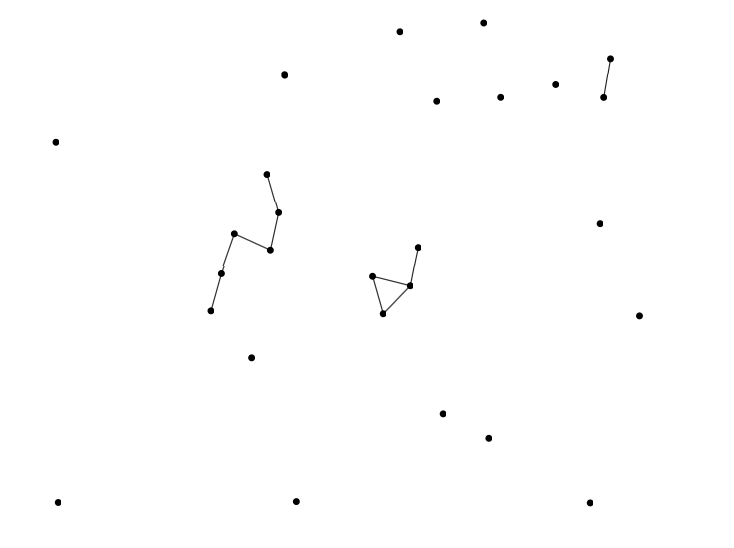
\includegraphics[width=7cm]{demo1.png}}
  \subfloat[]{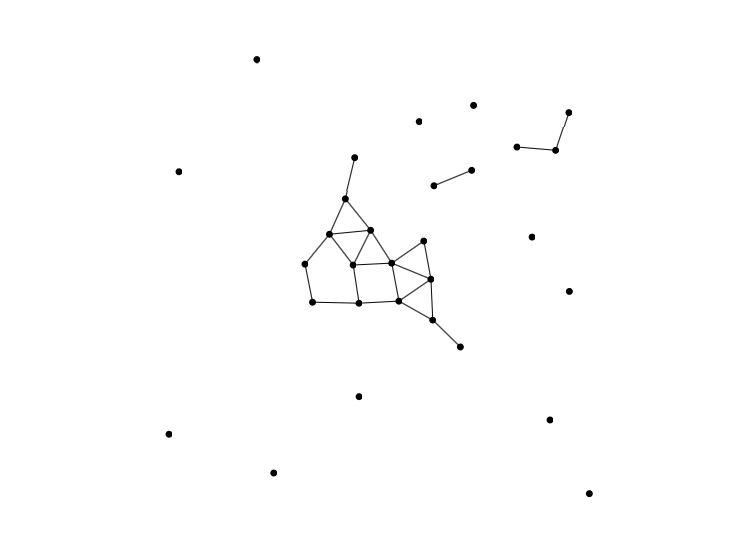
\includegraphics[width=7cm]{demo2.png}}\\
  \subfloat[]{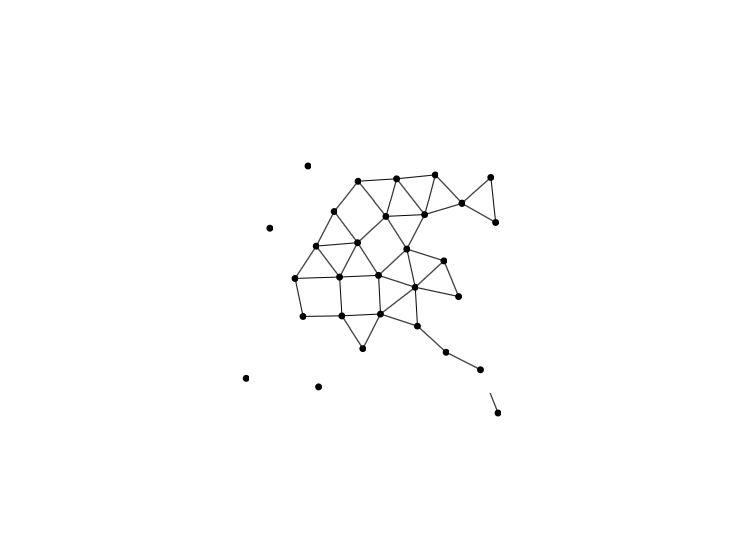
\includegraphics[width=7cm]{demo3.png}}
  \subfloat[]{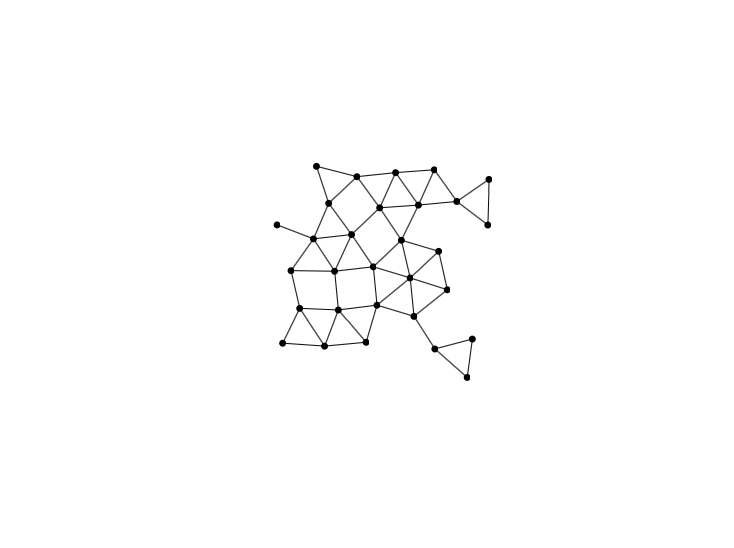
\includegraphics[width=7cm]{demo4.png}}\\
  \subfloat[]{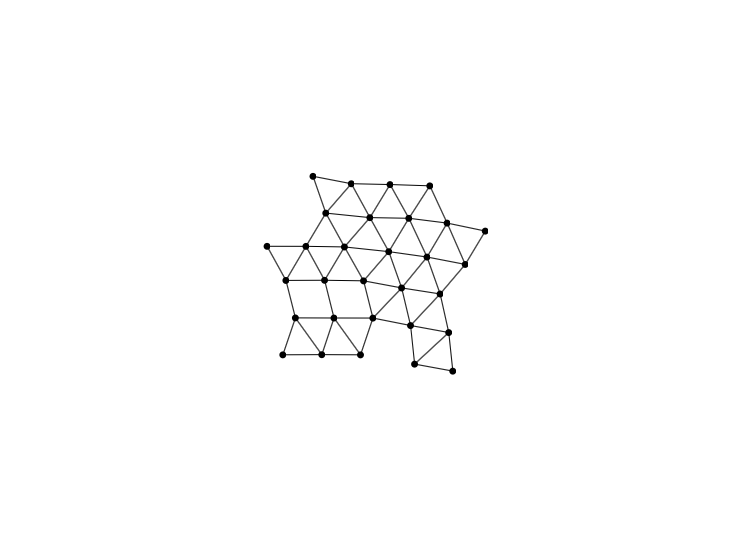
\includegraphics[width=7cm]{demo5.png}}

  \caption{Différentes étapes de la formation d'un réseau connexe.}
  \label{demo}

\end{figure}

\bibliographystyle{alpha}
\bibliography{references}

\end{document}
